\documentclass[a4paper,10pt]{article}

\usepackage[hidelinks]{hyperref}
\usepackage{float}
\usepackage{amsmath}
\usepackage{fixltx2e} % (vecchio)

% Lingua
\usepackage[utf8]{inputenc}
\usepackage[italian]{babel}

% Margini
\usepackage{geometry}
\geometry{a4paper, top=3cm, bottom=3cm, left=3cm, right=3cm}
\setlength{\parindent}{0pt}

\usepackage{graphicx}   % per immagini
\usepackage{hyperref}   % per link
\usepackage{caption}    % per didascalie
\captionsetup[table]{labelformat=empty}
\usepackage{ifthen}     % per \ifthenelse

\usepackage{tikz}

\usepackage{array}      % per tabelle
\newcolumntype{M}[1]{>{\centering\arraybackslash}m{#1}}

\usepackage{datetime}

% Definisci un formato personalizzato
\newdateformat{italianformat}{\THEDAY~\monthname[\THEMONTH]~\THEYEAR}
\newdate{dataverbale}{12}{01}{2026}

% Definizione del formato con le barre
\newdateformat{slashdate}{\twodigit{\THEDAY}/\twodigit{\THEMONTH}/\THEYEAR}

% Per logo in ogni pagina
\usepackage{eso-pic}
\usepackage{tikz}
\AddToShipoutPictureBG{%
  \ifthenelse{\value{page}>1}{%
    \begin{tikzpicture}[remember picture, overlay]
      % Icona
      \node[anchor=north west, inner sep=0pt] at ([xshift=28pt,yshift=-28pt]current page.north west) 
        {
\includegraphics[width=1cm, height=1cm]{resources/Tool-8_icon_white.png}};
      
      % Riga
      \draw[black, line width=0.5pt] ([xshift=28pt + 1cm, yshift=-28pt - 0.6cm]current page.north west) 
            -- ++(3cm, 0);
      % Testo
      \node[anchor=west, text=black, font=\small] at ([xshift=28pt + 1cm, yshift=-28pt - 0.4cm]current page.north west) 
        {Piano di Qualifica};
    \end{tikzpicture}
  }{}
}


%------Ridefinizione maketitle-------
\makeatletter
\renewcommand{\maketitle}{%
  \vspace*{\fill}
  \begin{center}
    {\LARGE \bfseries \@title \par}
    \vskip 1em
    {\large \@author \par}
    \vskip 1em
    {\large\slashdate{\displaydate{dataverbale}} \par}
  \end{center}
  \vspace*{\fill}
}
\makeatother
%-----------------------------------

\title{%
  
\includegraphics[width=10cm]{resources/Tool-8_white_2.png} \\[1.5ex]
  \textbf{\LARGE Piano di Qualifica}
}
\author{}
\date{\dataverbale}
\begin{document}
\tikz[remember picture,overlay] \node[opacity=0.2,inner sep=0pt] at (current page.center){
\includegraphics[width=\paperwidth,height=\paperheight]{resources/Abstract_lines.png}};

\maketitle

\newpage

\section*{Revisioni}
\begin{table}[h!]
\centering
\begin{tabular}{|M{0.8cm}|p{3cm}|p{4.1cm}|M{1.8cm}|p{3cm}|}
  \hline
  \textbf{Ver.} & \textbf{Autore} & \textbf{Modifiche} & \textbf{Data} & \textbf{Verifica} \\
  \hline
  0.1 & Stefano Maso & Prima stesura documento completo & \slashdate{\displaydate{dataverbale}} & Besnik Murtezan \\
  \hline
\end{tabular}
\label{tab:revisioni}
\end{table}

\newpage

\tableofcontents

\newpage

\section{Introduzione}
\subsection{Scopo del documento}
Il Piano di Qualifica definisce le metriche di valutazione del prodotto, sulla base dei requisiti e delle aspettative della proponente, in modo da poter definire la qualità del prodotto attraverso un processo di continuo miglioramento.
Il Piano di Qualifica è concepito per essere incrementale e dinamico, soprattutto per quanto riguarda le metriche descritte e punta a dare una valutazione il più oggettiva possibile di ciò che è stato realizzato. Eventuali termini tecnici sono definiti all'interno del documento "Glossario".
\subsection{Riferimenti}
\subsubsection{Riferimenti normativi}
\begin{itemize}
    \item Norme di Progetto$^G$
    \item Capitolato$^G$ C6 - Progetto Second Brain:    \\ \url{https://www.math.unipd.it/~tullio/IS-1/2025/Progetto/C6.pdf}
\end{itemize}
\subsubsection{Riferimenti informativi}
\begin{itemize}
    \item Lezione \textit{Progettazione Software (T6)} del corso di \textit{Ingegneria del software$^G$}: \\ \url{https://www.math.unipd.it/~tullio/IS-1/2025/Dispense/T06.pdf}
    \item Lezione \textit{Qualità di prodotto (T7)} del corso di \textit{Ingegneria del software}: \\ \url{https://www.math.unipd.it/~tullio/IS-1/2025/Dispense/T0.pdf}
    \item Lezione \textit{Qualità di processo (T8)} del corso di \textit{Ingegneria del software}: \\ \url{https://www.math.unipd.it/~tullio/IS-1/2025/Dispense/T08.pdf}
    \item Lezione \textit{Verifica e validazione: introduzione (T9)} del corso di \textit{Ingegneria del software}: \\ \url{https://www.math.unipd.it/~tullio/IS-1/2025/Dispense/T09.pdf}
    \item Lezione \textit{Verifica e validazione: analisi statica (T10)} del corso di \textit{Ingegneria del software}: \\ \url{https://www.math.unipd.it/~tullio/IS-1/2025/Dispense/T10.pdf}
    \item Lezione \textit{Verifica e validazione: analisi dinamica aka testing (T11)} del corso di \textit{Ingegneria del software}: \\ \url{https://www.math.unipd.it/~tullio/IS-1/2025/Dispense/T11.pdf}
    \item Metriche di progetto (\textit{Earned Value Analysis}): \\ \url{https://it.wikipedia.org/wiki/Metriche_di_progetto}
\end{itemize}
\subsection{Codifica delle metriche}
Una metrica è identificata dal seguente formato di codice: 
\begin{center}
    [Tipo][Id]-[Acronimo]
\end{center}
\begin{itemize}
    \item \textbf{Tipo}: può essere PC (per un processo) o PD (per un prodotto)
    \item \textbf{Id}: identificativo all'interno di un certo tipo di metrica
    \item \textbf{Acronimo}: acronimo del nome della metrica
\end{itemize}
Ogni metrica avrà una descrizione, i valori accettabili e quelli preferibili.

\section{Qualità di processo}
La qualità è determinata dai processi che la compongono, misurata scegliendo delle buone metriche di misurazione di qualità e anche buoni strumenti (serve automazione e oggettività). 
\subsection{Processi primari}
\subsubsection{Fornitura}
Per definire le metriche adottate per i processi primari di fornitura andremo a fare riferimento alla tecnica denominata \textit{EVA} (\textit{Earned Value Analysis}) che consenste di calcolare in termini di tempo, denaro speso e valore del lavoro realizzato e di valutare le performance del progetto.\\ Tra queste individuiamo:
\begin{itemize}
    \item \textbf{Budget at Completion (BAC)}: valore previsto inizialmente per la realizzazione del progetto
    \item \textbf{Estimated at Completion (EAC)}: revisione del valore stimato per la realizzazione del progetto
    \item \textbf{Planned Value (PV)}: costo previsto per realizzare le attività di progetto per la data stabilita (tempo o denaro)
    \item \textbf{Actual Cost (AC)}: costo effettivamente sostenuto alla data stabilita (tempo o denaro)
    \item \textbf{Earned Value (EV)}: valore delle attività sostenute alla data stabilita (tempo o denaro)
    \item \textbf{Estimated to Complete (ETC)}: valore stimato per completare le attività rimanenti necessarie per concludere il progetto
    \item \textbf{Cost Variance (CV)}: misura la variazione del valore ottenuto (EV) rispetto al costo effettivo (AC)
    \item \textbf{Schedule Variance (SV)}: misura la variazione del valore ottenuto (EV) rispetto al costo pianificato (PV)
    \item \textbf{Budget Variance (BV)}: misura la variazione dal costo attuale (AC) rispetto al costo atteso (CV)
\end{itemize}
Come riportato dal documento Dichiarazione di Impegni, il BAC corrisponde ad un valore di \textbf{€ 10.950,00}.
\\
Obiettivi di qualità per tali metriche: 
\begin{table}[H]
\centering
\renewcommand{\arraystretch}{1.2}
\begin{tabular}{|l|l|c|c|}
\hline
\textbf{Metrica} & \textbf{Nome} & \textbf{Valore Accettabile} & \textbf{Valore Preferibile} \\
\hline
PC01-EAC & Estimated at Completion & $\pm 5\%$ BAC & = BAC \\
PC02-PV  & Planned Value           & $\geq 0$      & $\leq$ BAC \\
PC03-AC  & Actual Cost             & $\geq 0$      & $\leq$ EAC \\
PC04-EV  & Earned Value             & $\geq 0$      & $\leq$ EAC \\
PC05-ETC & Estimated to Complete    & $\geq 0$      & $\leq$ EAC \\
PC06-CV  & Cost Variance            & $\geq -7.5\%$ & $\geq 0$ \\
PC07-SV  & Schedule Variance        & $\geq -7.5\%$ & $\geq 0$ \\
PC08-BV  & Budget Variance          & $\pm 10\%$    & = 0 \\
\hline
\end{tabular}
\caption{Metriche per i processi di fornitura}
\label{tab:metriche-fornitura}
\end{table}
\subsubsection{Sviluppo}
\textbf{Analisi dei Requisiti} Per l'attività di \textit{Analisi dei Requisiti$^G$} definiamo le seguenti metriche:
\begin{itemize}
    \item \textbf{Requirements stability index (RSI)}: misura la stabilità dei requisiti nel corso del tempo durante lo sviluppo del progetto; è misurata nel suguente modo:
    \begin{center}
        \[
        RSI = 1 - \left( \frac{N_{\text{modifiche}}}{N_{\text{requisiti totali}}} \right) \times 100
        \]
    \end{center}
    Dove: \\
    - N\textsubscript{modifiche} è il numero totale di modifiche apportate ai requisiti durante un periodo di tempo specifico \\
    - N\textsubscript{requisiti totali} è il numero totale di requisiti del progetto
\end{itemize}
\textbf{Progettazione} Per l'attività di progettazione definiamo le seguenti metriche:
\begin{itemize}
    \item \textbf{Structural fan-in (SFIN)}: misura la quantità dei moduli che utilizzano un modulo specifico, un valore alto significa che molte parti del sistema dipendono da un modulo in particolare
    \item \textbf{Structural fan-out (SFOUT)}: misura il numero di moduli utilizzati da un modulo specifico, un valore alto significa che il modulo considerato dipende da molti altri moduli
\end{itemize}
\textbf{Codifica} Per l'attività di codifica definiamo le seguenti metriche:
\begin{itemize}
    \item \textbf{Linee di codice (LOC)}: misura la complessità del software in base al numero di linee di codice sorgente
\end{itemize}
Obiettivi per tali metriche:
\begin{table}[H]
\centering
\renewcommand{\arraystretch}{1.2}
\begin{tabular}{|l|l|c|c|}
\hline
\textbf{Metrica} & \textbf{Nome} & \textbf{Valore Accettabile} & \textbf{Valore Preferibile} \\
\hline
PC09-RSI & Requirements stability index & $\geq 70\%$ & $100\%$ \\
PC10-SFIN  & Structural fan-in           & -      & Masismo \\
PC11-SFOUT  & Structural fan-out            & -      & Minimo \\
PC12-LOC  & Linee di codice             & $\leq 50.000$      & $\leq 30.000$  \\
\hline
\end{tabular}
\caption{Metriche per i processi di sviluppo}
\label{tab:metriche-sviluppo}
\end{table}

\subsection{Processi di supporto}
\subsubsection{Documentazione} 
Per il processo di documentazione definiamo le seguenti metriche:
\begin{itemize}
    \item \textbf{Errori ortografici (EO)}: misura la quantità di errori ortografici individuati per documento
    \item \textbf{Indice Gulpease (IG)}: misura la leggibilità di un documento in lingua italiana, calcolato nel seguente modo:
        \[
        IG = 89 + \frac{300 \times (num. frasi) - 10 \times (num. lettere) }{num. parole}
        \]
    Dove: \\
    - \textit{num. frasi} è il numero di frasi nel documento \\
    - \textit{num. lettere} è il numero di lettere nel documento \\
    - \textit{num. parole} è il numero di parole nel documento
\end{itemize}
Obiettivi per tali metriche:
\begin{table}[H]
\centering
\renewcommand{\arraystretch}{1.2}
\begin{tabular}{|l|l|c|c|}
\hline
\textbf{Metrica} & \textbf{Nome} & \textbf{Valore Accettabile} & \textbf{Valore Preferibile} \\
\hline
PC13-EO & Errori ortografici & 0 & 0 \\
PC14-IG  & Indice Gulpease & 30-100      & 50-100 \\
\hline
\end{tabular}
\caption{Metriche per i processi di supporto}
\label{tab:metriche-supporto}
\end{table}
\subsection{Processi organizzativi}
Per i processi organizzativi definiamo le seguenti metriche:
\begin{itemize}
    \item \textbf{Non Calculated Risk (NCR)}: misura la quantità di rischi non previsti o non stimati
    \item \textbf{Efficienza temporale (ET)}: misura quanto tempo viene impiegato per attività produttive rispetto alle ore individuali:
    \[
    ET = \frac{\text{Ore individuali}}{\text{Ore produttive}}
    \]
    Dove: \\
    - \textit{Ore individuali} sono le ore che portano al raggiungimento di obiettivi \\
    - \textit{Ore produttive} rappresentano il tempo totale trascorso come ore di orologio
\end{itemize}
Obiettivi per tali metriche:
\begin{table}[H]
\centering
\renewcommand{\arraystretch}{1.2}
\begin{tabular}{|l|l|c|c|}
\hline
\textbf{Metrica} & \textbf{Nome} & \textbf{Valore Accettabile} & \textbf{Valore Preferibile} \\
\hline
PC15-NCR & Non Calculated Risk & $\leq 4$ & 0 \\
PC16-ET  & Efficienza temporale  & $\leq 3$ & $\leq 1$ \\
\hline
\end{tabular}
\caption{Metriche per i processi organizzativi}
\label{tab:metriche-organizzativi}
\end{table}




\section{Qualità di prodotto}
Questa sezione è dedicata agli obiettivi che un prodotto software di qualità dovrebbe avere. Ecco gli obiettivi di qualità esterni:
\begin{itemize}
    \item \textit{Adeguatezza funzionale}: cioè la capacità di fornire le funzionalità e le caratteristiche previste, soddisfando i requisiti funzionali
    \item \textit{Efficienza}: la capacità di fornire prestazioni adeguate e di utilizzo delle risorse di sistema
    \item \textit{Usabilità}: cioè la misura all'apprendimento, comprensione e operabilità del prodotto da parte dell'utente
    \item \textit{Affidabilità}: misura la capacità del prodotto di funzionare correttamente sotto determinate condizioni
    \item \textit{Sicurezza}: la capacità del software di proteggere dati sensibili e prevenire accessi non autorizzati
\end{itemize}
Gli obiettivi di qualità interni:
\begin{itemize}
    \item \textit{Manutenibilità}: misura la facilità con cui il prodotto può essere modificato, aggiornato e corretto
    \item \textit{Portabilità}: misura la facilità con cui il prodotto può essere trasferito da un ambiente ad un altro
\end{itemize}
\subsection{Adeguatezza funzionale}
Per l'adeguatezza funzionale useremo le seguente metrica:
\begin{itemize}
    \item \textbf{Copertura dei requisiti obbligatori (CRO)}: misura la percentuale dei requisiti obbligatori soddisfatti
    \[
        CRO = \frac{N_{ros}}{N_{rot}} \times 100
    \]
    Dove:  \\
    - N\textsubscript{ros} rappresentano il numero di requisiti obbligatori soddisfatti \\
    - N\textsubscript{rot} rappresentano il numero di requisiti obbligatori totali
\end{itemize}
Obiettivi di qualità per tale metrica: 
\begin{table}[H]
\centering
\renewcommand{\arraystretch}{1.2}
\begin{tabular}{|l|l|c|c|}
\hline
\textbf{Metrica} & \textbf{Nome} & \textbf{Valore Accettabile} & \textbf{Valore Preferibile} \\
\hline
PD01-CRO & Copertura dei requisiti obbligatori & $100\%$ & $100\%$ \\
\hline
\end{tabular}
\caption{Metriche per l'adeguatezza funzionale}
\label{tab:metriche-adfunzionale}
\end{table}
\subsection{Efficienza}
Per l'efficienza usiamo la seguente metrica:
\begin{itemize}
    \item \textbf{Tempo di risposta medio (TM)}: misura il tempo impiegato dal software di gestire ed elaborare una richiesta fino al risultato finale
\end{itemize}
Obiettivi per tale metrica:
\begin{table}[H]
\centering
\renewcommand{\arraystretch}{1.2}
\begin{tabular}{|l|l|c|c|}
\hline
\textbf{Metrica} & \textbf{Nome} & \textbf{Valore Accettabile} & \textbf{Valore Preferibile} \\
\hline
PD02-TM & Tempo di risposta medio & 3 secondi & 2 secondi \\
\hline
\end{tabular}
\caption{Metriche per l'efficienza}
\label{tab:metriche-efficienza}
\end{table}
\subsection{Usabilità}
Per l'usabilità usiamo le seguenti metriche:
\begin{itemize}
    \item \textbf{Tempo di apprendimento (TA)}: misura il tempo impiegato dall'utente di imparare e utilizzare le funzionalità del software 
    \item \textbf{Raggiunta dell'obiettivo (RO)}: misura il numero di iterazioni necessarie all'utente per raggiungere il risultato voluto
    \item \textbf{Errori dell'utente (EU)}: misura il numero di errori che l'utente compie prima di raggiungere l'obiettivo desiderato 
\end{itemize}
Obiettivi per tali metriche:
\begin{table}[H]
\centering
\renewcommand{\arraystretch}{1.2}
\begin{tabular}{|l|l|c|c|}
\hline
\textbf{Metrica} & \textbf{Nome} & \textbf{Valore Accettabile} & \textbf{Valore Preferibile} \\
\hline
PD03-TA & Tempo di apprendimento & 20 minuti & 10 minuti \\
PD04-RO & Raggiunta dell'obiettivo & 7 click & 4 click \\
PD05-EU & Errori dell'utente & 3 & 0 \\
\hline
\end{tabular}
\caption{Metriche per l'usabilità}
\label{tab:metriche-usabilità}
\end{table}
\subsection{Affidabilità}
Per l'affidabilità useremo la seguente metrica:
\begin{itemize}
    \item \textbf{Failure density (FD)}: misura in percentuale l'affidabilità del software
    \[
    FD = \frac{N_{tf}}{N_{te}} \times 100
    \]
    Dove: \\
    - N\textsubscript{tf} rappresentano il numero di testi falliti \\
    - N\textsubscript{te} rappresentano il numero di test effettuati 
\end{itemize}
Obiettivi per tale metrica:
\begin{table}[H]
\centering
\renewcommand{\arraystretch}{1.2}
\begin{tabular}{|l|l|c|c|}
\hline
\textbf{Metrica} & \textbf{Nome} & \textbf{Valore Accettabile} & \textbf{Valore Preferibile} \\
\hline
PD06-FD & Failure density & $10\%$ & $0\%$ \\
\hline
\end{tabular}
\caption{Metriche per l'affidabilità}
\label{tab:metriche-affidabilità}
\end{table}
\subsection{Manutenibilità}
Per la manutenibilità andremo ad usare la seguente metrica:
\begin{itemize}
    \item \textbf{Complessità ciclomatica (CC)}: misura la complessità del software utilizzando il grafo di controllo del flusso
    \[
    v(G) = e - n + p
    \]
    Dove: \\
    - G rappresenta il grafo \\
    - e rappresenta il numero di archi in G \\
    - n rappresenta il numero di nodi in G \\
    - p rappresenta il numero delle componenti connesse da ogni arco 
\end{itemize}
Obiettivi per tale metrica:
\begin{table}[H]
\centering
\renewcommand{\arraystretch}{1.2}
\begin{tabular}{|l|l|c|c|}
\hline
\textbf{Metrica} & \textbf{Nome} & \textbf{Valore Accettabile} & \textbf{Valore Preferibile} \\
\hline
PD07-CC & Complessità ciclomatica & $\leq 15$ & $\leq 10$ \\
\hline
\end{tabular}
\caption{Metriche per la manutenibilità}
\label{tab:metriche-manutenibilità}
\end{table}
\subsection{Portabilità}
Per la portabilità andremo ad usare la seguente metrica:
\begin{itemize}
    \item \textbf{Browser supportati (BS)}: misura in percentuale le versioni dei browser supportati
    \[ 
        BS = \frac{N_{vbs}}{N_{vbp}} \times 100
    \]
    Dove: \\
    - N\textsubscript{vbs} rappresenta il numero di versioni di browser supportate \\
    - N\textsubscript{vbp} rappresenta il numero di versioni di browser previste da supportare
\end{itemize}
Obiettivi per tale metrica:
\begin{table}[H]
\centering
\renewcommand{\arraystretch}{1.2}
\begin{tabular}{|l|l|c|c|}
\hline
\textbf{Metrica} & \textbf{Nome} & \textbf{Valore Accettabile} & \textbf{Valore Preferibile} \\
\hline
PD08-BS & Browser supportati & $100\%$ & $100\%$ \\
\hline
\end{tabular}
\caption{Metriche per la portabilità}
\label{tab:metriche-portabilità}
\end{table}

\section{Testing}
In questa sezione verranno esplorate le metodologie di testing e la loro specifica. L'obiettivo è seguire il "\textit{Modello a V$^G$}", in cui ad ogni fase di sviluppo corrisponde un tipo di test da eseguire.\\
I test di dividono in:
\begin{itemize}
    \item \textbf{Test di unità}: vengono eseguiti sulle unità più semplici del codice e viene fatta corrispondere all'attività di codifica
    \item \textbf{Test di integrazione}: vengono eseguiti per verificare la corretta integrazione tra le diverse unità software e viene fatta corrispondere all'attività di progettazione
    \item \textbf{Test di sistema}: verificando il funzionamento corretto dell'intero sistema e soprattutto che tutti i requisiti siano soddisfatti; viene fatta corrispondere all'attività di \textit{Analisi dei Requisiti}
    \item \textbf{Test di accettazione}: verificando, alla presenza del committente, che il prodotto finale soddisfi tutti i requisiti, se questo test risulta superato si può procedere al rilascio
\end{itemize}
\subsection{Test di sistema}
I test di sistema hanno lo scopo di verificare che il sistema software rispetti i requisiti specificati nel documento "\textit{Analisi dei Requisiti}". In seguito verranno elencati i vari test, i quali avranno un codice identificativo, una descrizione, il requisito a cui fa riferimento e lo stato del test. \\
*TABELLA DEI REQUISITI DA FARE!!!*


\section{Checklist}
La verifica tramite analisi statica è preferibile che avvenga tramite \textit{Inspection} anzichè \textit{Walkthrough}, proprio per questo motivo vengono definite delle liste di controllo (aggiornate progressivamente dai verificatori) che permettono di analizzare velocemente gli errori più comuni.
\subsection{Documentazione}
\subsubsection{Struttura}
\begin{table}[H]
\centering
\renewcommand{\arraystretch}{1.2}
\begin{tabular}{|p{4cm}|p{9cm}|}
\hline
\textbf{Errore} & \textbf{Descrizione} \\
\hline
Manca la \textit{caption$^G$} per le tabelle o le immagini &
Ogni tabella o immagine deve possedere una \textit{caption}. \\
\hline
Sezione vuota &
Le sezioni vuote devono essere eliminate. \\
\hline
\end{tabular}
\caption{Checklist dei possibili errori nella struttura della documentazione}
\label{tab:checklist-struttura}
\end{table}
\subsubsection{Errori ortografici}
\begin{table}[H]
\centering
\renewcommand{\arraystretch}{1.2}
\begin{tabular}{|p{4cm}|p{9cm}|}
\hline
\textbf{Errore} & \textbf{Descrizione} \\
\hline
Errore di sintassi & Errori di battitura o distrazione devono essere rimossi \\
\hline
Errore di coniugazione & Gli errori di coniugazione devono essere rimossi \\
\hline
\end{tabular}
\caption{Checklist dei possibili errori ortografici nella documentazione}
\label{tab:checklist-ortografia}
\end{table}

\subsubsection{Analisi dei Requisiti}
\begin{table}[H]
\centering
\renewcommand{\arraystretch}{1.2}
\begin{tabular}{|p{4cm}|p{9cm}|}
\hline
\textbf{Errore} & \textbf{Descrizione} \\
\hline
Requisiti per un caso d'uso assenti & Ad ogni caso d'uso deve corrispondere almeno un requisito \\
\hline
Diagrammi dei casi d'uso$^G$ erronei & I diagrammi dei casi d'uso devono riportare la corretta numerazione e nomenclatura del caso d'uso stesso e riferirsi allo stesso modo ad altri casi d'uso \\
\hline
\end{tabular}
\caption{Checklist dei possibili errori per l'Analisi dei Requisiti}
\label{tab:checklist-analisi}
\end{table}

\section{Cruscotto di valutazione della qualità}
\subsection{PC01-EAC (Estimated at Completion)}
\begin{figure}[H]
    \centering
    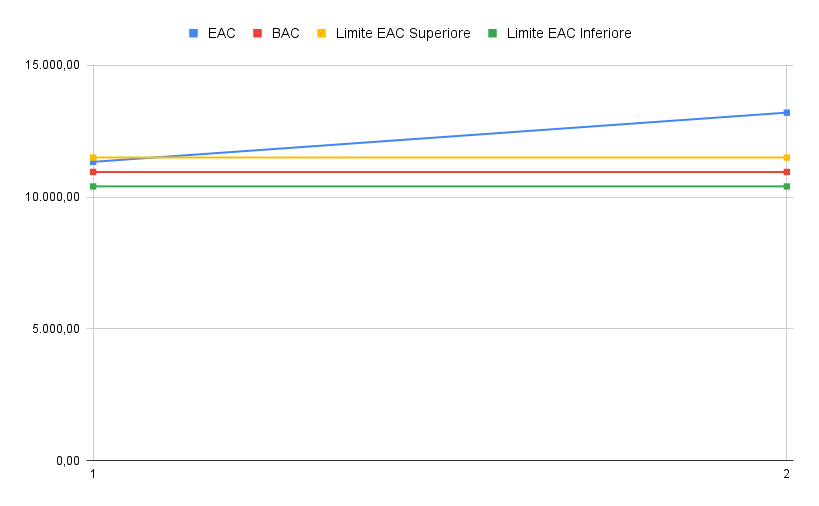
\includegraphics[width=0.9\linewidth]{resources/chart.png}
    \caption{Estimated at Completion}
\end{figure}
Dal grafico si può notare come l'EAC superi il valore accettabile di quest'ultimo. La causa di questa situazione è riconducibile ad una scorretta divisione tra ore produttive e individuali. Dopo la fase iniziale il gruppo dovrebbe riuscire a rientrare nei valori ottimali. Il team è consapevole che l'andamento è dovuto ad una gestione errata del progetto, perciò tutti i membri dovranno impegnarsi per rientrare nel valore ottimale.

\subsection{PC02-PV (Planned Value) e PC04-EV (Earned Value)}
\begin{figure}[H]
    \centering
    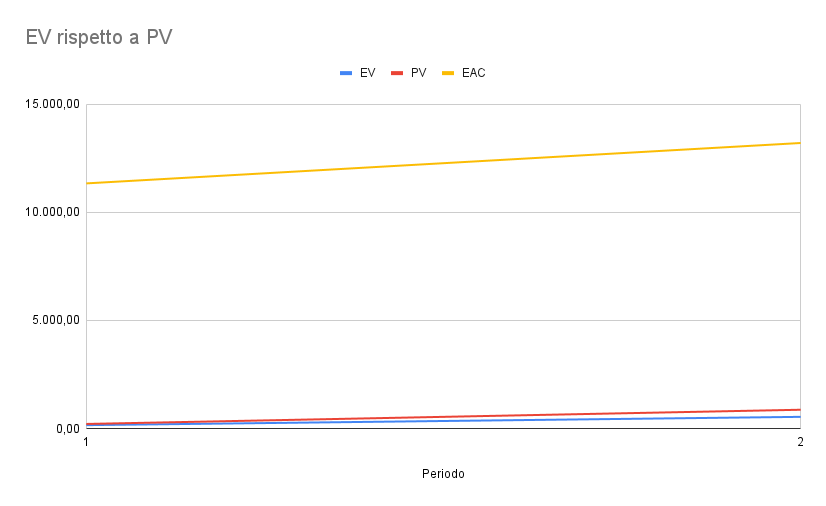
\includegraphics[width=0.9\linewidth]{resources/EV rispetto a PV.png}
    \caption{Planned Value - Earned Value}
\end{figure}
Le linee del PV e dell'EV sono vicine, ma dall'ultimo periodo si stanno allontanando, il dovrà dunque impegnarsi maggiormente per svolgere ad ogni periodo quanto pianificato.

\subsection{PC05-ETC (Estimated to Complete)}
\begin{figure}[H]
    \centering
    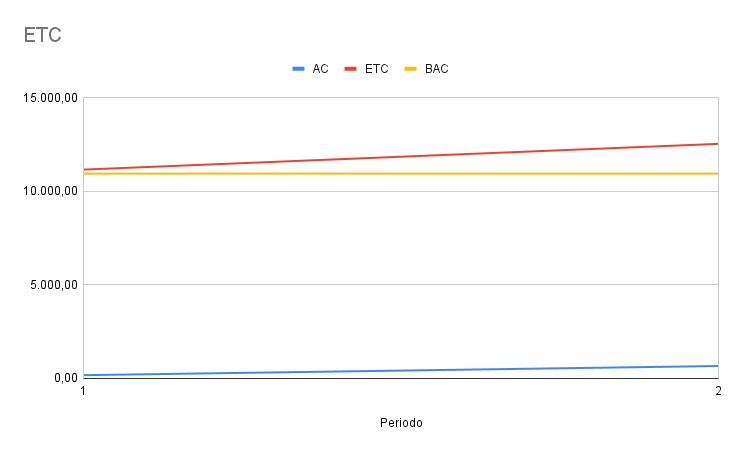
\includegraphics[width=0.9\linewidth]{resources/ETC.png}
    \caption{Estimated to Complete}
\end{figure}
Dal grafico si evince che è necessario produrre più valore in ciascun periodo in modo da rientrare nel costo pianificato.

\subsection{PC06-CV (Cost Variance), PC07-SV (Schedule Variance) e PC08-BV (Budget Variance)}
\begin{figure}[H]
    \centering
    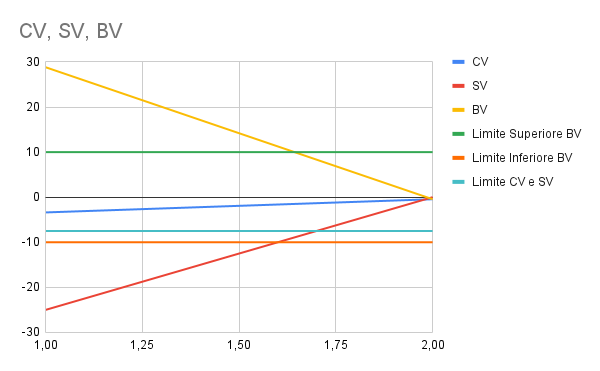
\includegraphics[width=0.9\linewidth]{resources/CV, SV, BV.png}
    \caption{Cost Variance, Schedula Variance e Budget Variance}
\end{figure}
Dopo un primo periodo in cui sia il Budget Variance chche lo Schedule Variance erano lontanissimi dal valore preferibile, siamo giunti a un buon punto. Allo stesso modo, la Cost Variance si sta avvicinando al valore preferibile.

\section{Valutazioni per il miglioramento}
Questa sezione è dedicata alla valutazione generale del lavoro, con lo scopo di inserire osservazioni sui problemi riscontrati e sulle possibili correzioni da adottare.
\subsection{Valutazione sull'organizzazione}
\begin{table}[H]
\centering
\renewcommand{\arraystretch}{1.2}
\begin{tabular}{|p{3cm}|p{4cm}|p{2cm}|p{4cm}|}
\hline
\textbf{Problema} & \textbf{Descrizione} & \textbf{Gravità} & \textbf{Soluzione} \\
\hline
Tracciamento temporale &
Inizialmente è stato difficile tracciare le ore per ogni attività del ruolo coperto da ogni membro &
Media &
Utilizzo di issue su GitHub$^G$ per suddividere ogni attività in base allo sprint, con relativo tracciamento temporale \\
\hline
\end{tabular}
\caption{Valutazione sull’organizzazione}
\label{tab:valutazione-organizzazione}
\end{table}

\subsection{Valutazione degli strumenti utilizzati}
\begin{table}[H]
\centering
\renewcommand{\arraystretch}{1.2}
\begin{tabular}{|p{3cm}|p{4cm}|p{2cm}|p{4cm}|}
\hline
\textbf{Problema} & \textbf{Descrizione} & \textbf{Gravità} & \textbf{Soluzione} \\
\hline
Suddivisione task &
Il gruppo ha spesso riscontrato problemi sulla divisione di task &
Bassa &
Creazione di sub-issue in modo da assegnare allo specifico membro la sua parte di issue da eseguire \\
\hline
\end{tabular}
\caption{Valutazione degli strumenti utilizzati}
\label{tab:valutazione-strmenti}
\end{table}

\subsection{Valutazione sui ruoli}
\begin{table}[H]
\centering
\renewcommand{\arraystretch}{1.2}
\begin{tabular}{|p{3cm}|p{4cm}|p{2cm}|p{4cm}|}
\hline
\textbf{Problema} & \textbf{Descrizione} & \textbf{Gravità} & \textbf{Soluzione} \\
\hline
Responsabile &
La partizione dei compiti e la gestione delle ore, prima dell'utilizzo delle issue su GitHub, era vaga e poco accurata &
Media &
Grazie alle issue su GitHub è possibile possibile tenere traccia delle ore impiegatate per ciascun task e quindi fare il resoconto dei costi e dei tempi rispetto al preventivo \\
\hline
\end{tabular}
\caption{Valutazione sui ruoli}
\label{tab:valutazione-ruoli}
\end{table}

\end{document}
